% Mechanical Assembly Progress Report - Deployment System
\documentclass[12pt]{article}
\usepackage[margin=1in]{geometry}
\usepackage{graphicx}
\usepackage{caption}
\usepackage{float}

\title{Mechanical Assembly Progress Report\\Deployment System}
\author{0104C}
\date{\today}

\begin{document}

\maketitle

\section{Introduction}

This report documents the mechanical assembly process for the deployment system chassis. The assembly involved fabricating and integrating structural components to create a functional housing for the gear rack mechanism and servo motors that drive the deployment action.

\section{Assembly Progress}

\subsection{Rack Hole Modification}

Initial assembly revealed that the gear rack did not fit through the designated hole in the chassis component. Figure \ref{fig:sanding} shows the manual sanding process to enlarge the hole opening. This modification was necessary to ensure smooth linear motion of the rack through the chassis structure.

\begin{figure}[H]
\centering
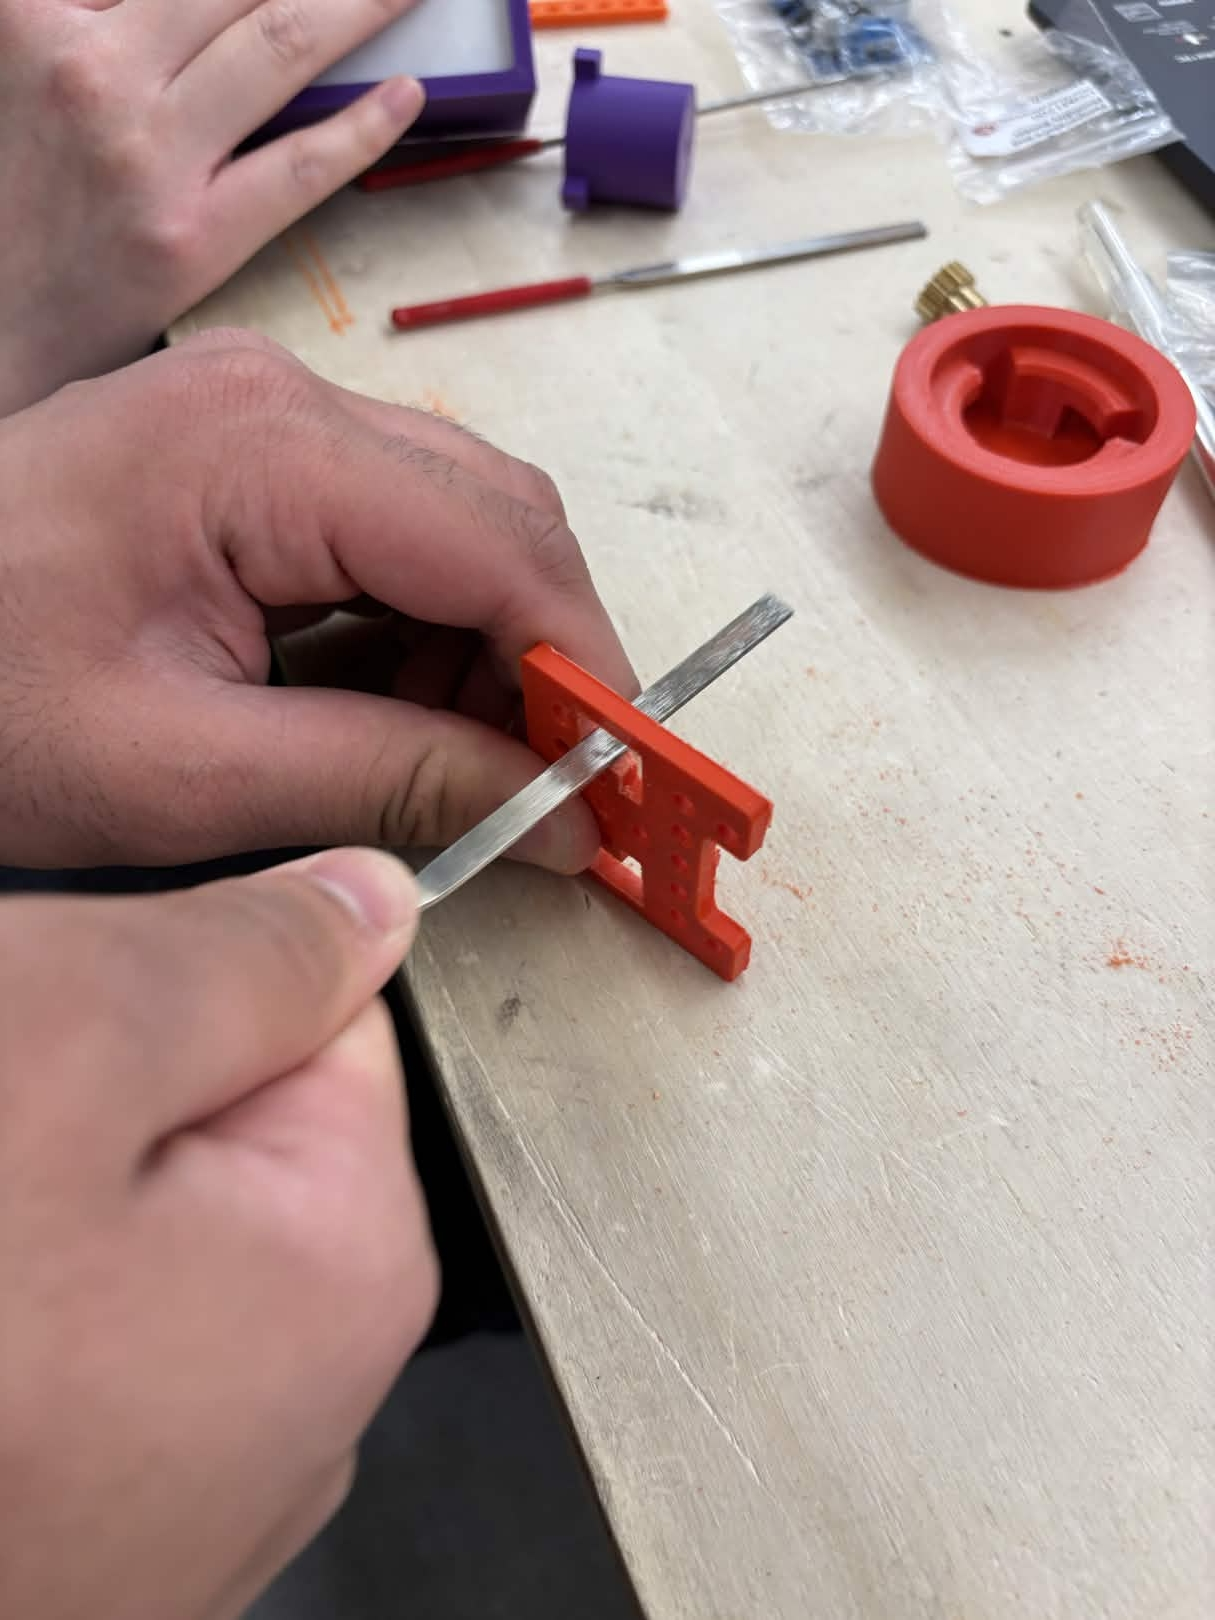
\includegraphics[width=0.65\textwidth]{../mech_img/sanding_rack_hole.jpg}
\caption{Sanding the rack hole to accommodate the gear rack clearance.}
\label{fig:sanding}
\end{figure}

\subsection{Chassis Assembly}

Following the modification, the chassis components were assembled as shown in Figure \ref{fig:assembling}. The red and blue structural plates were positioned to form the main chassis body, with mounting points aligned for the servo motors and gear mechanism. The orange gear rack was test-fitted to verify clearance.

\begin{figure}[H]
\centering
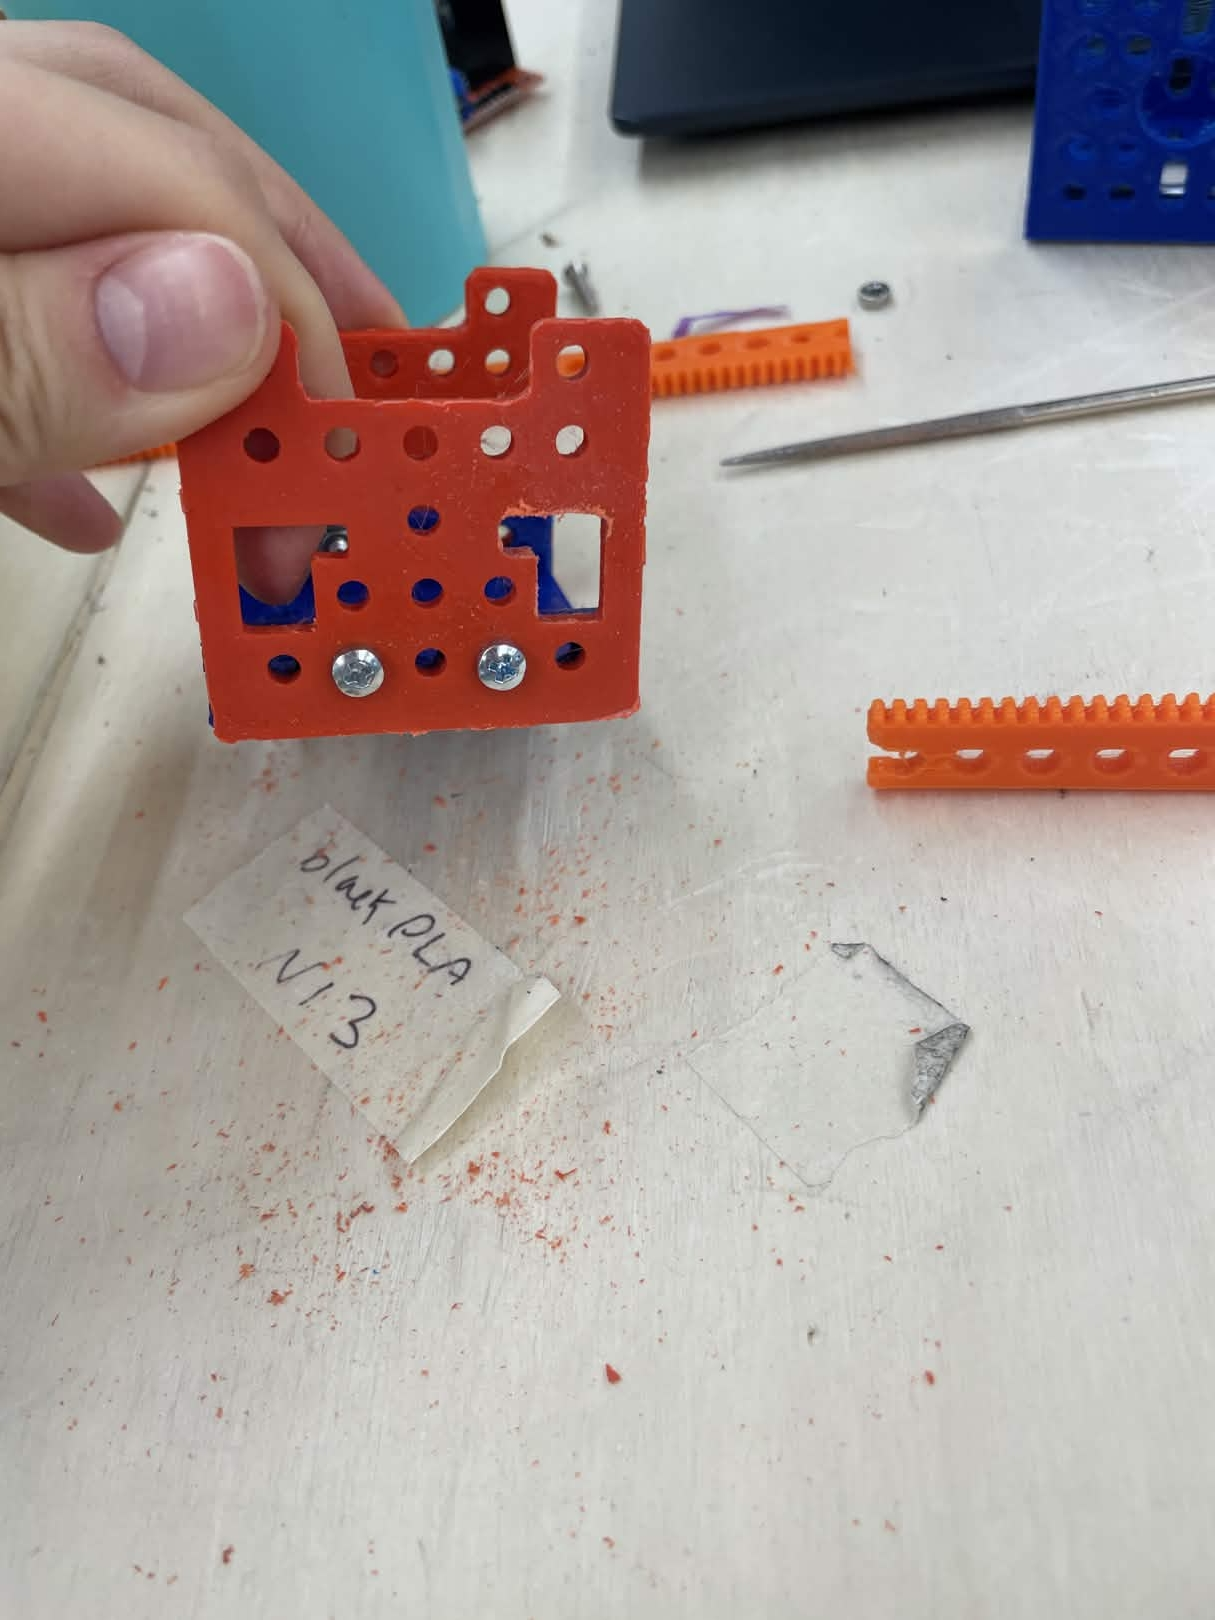
\includegraphics[width=0.65\textwidth]{../mech_img/assembling_chassis.jpg}
\caption{Assembling chassis components with gear rack test fit.}
\label{fig:assembling}
\end{figure}

\subsection{Securing Components}

The chassis components were secured using screws as depicted in Figure \ref{fig:screwing}. Fasteners were tightened to ensure rigid structural integrity while maintaining proper alignment of internal components. The servo motors were mounted within the chassis framework during this stage.

\begin{figure}[H]
\centering
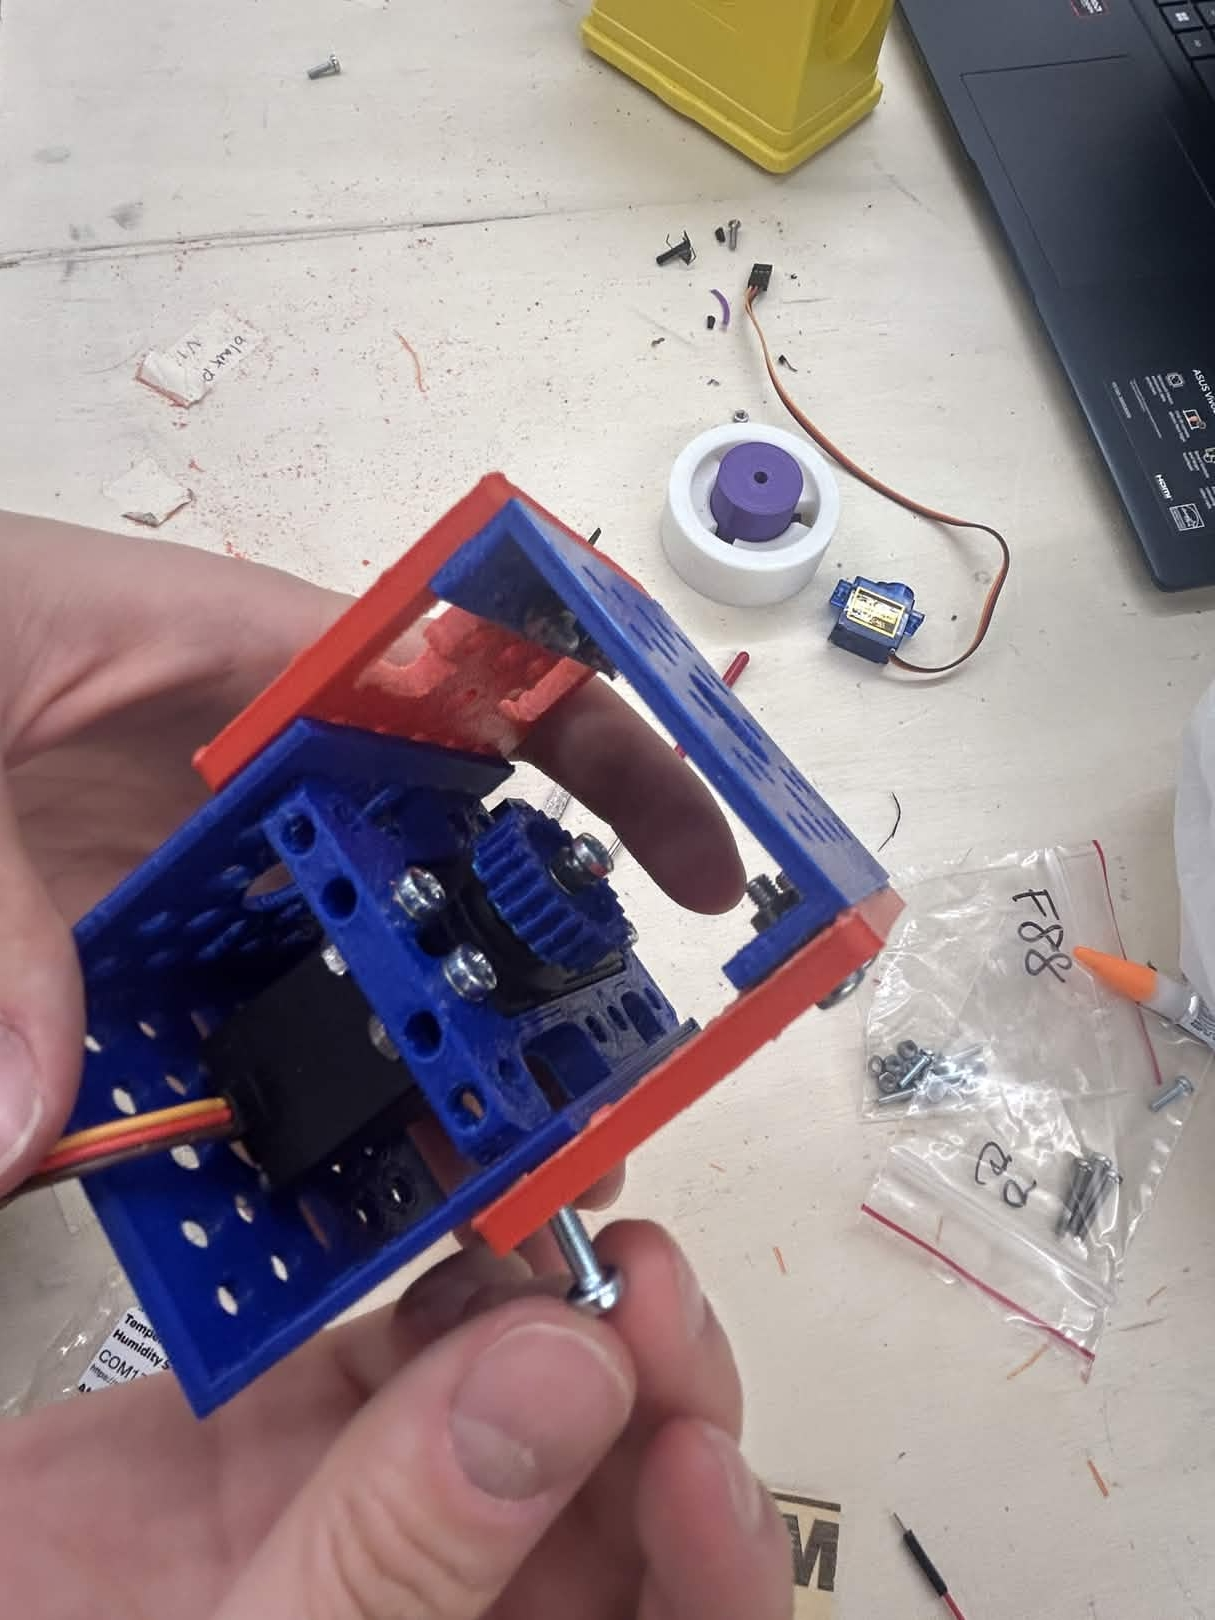
\includegraphics[width=0.65\textwidth]{../mech_img/screwing_chassis.jpg}
\caption{Securing chassis components with screws and mounting servo motors.}
\label{fig:screwing}
\end{figure}

\subsection{Pre-Integration Assembly}

Figure \ref{fig:assembled} shows the completed chassis assembly before gear rack insertion. The structural framework is fully secured, servo motors are mounted and wired, and the chassis is ready for final integration with the gear rack mechanism.

\begin{figure}[H]
\centering
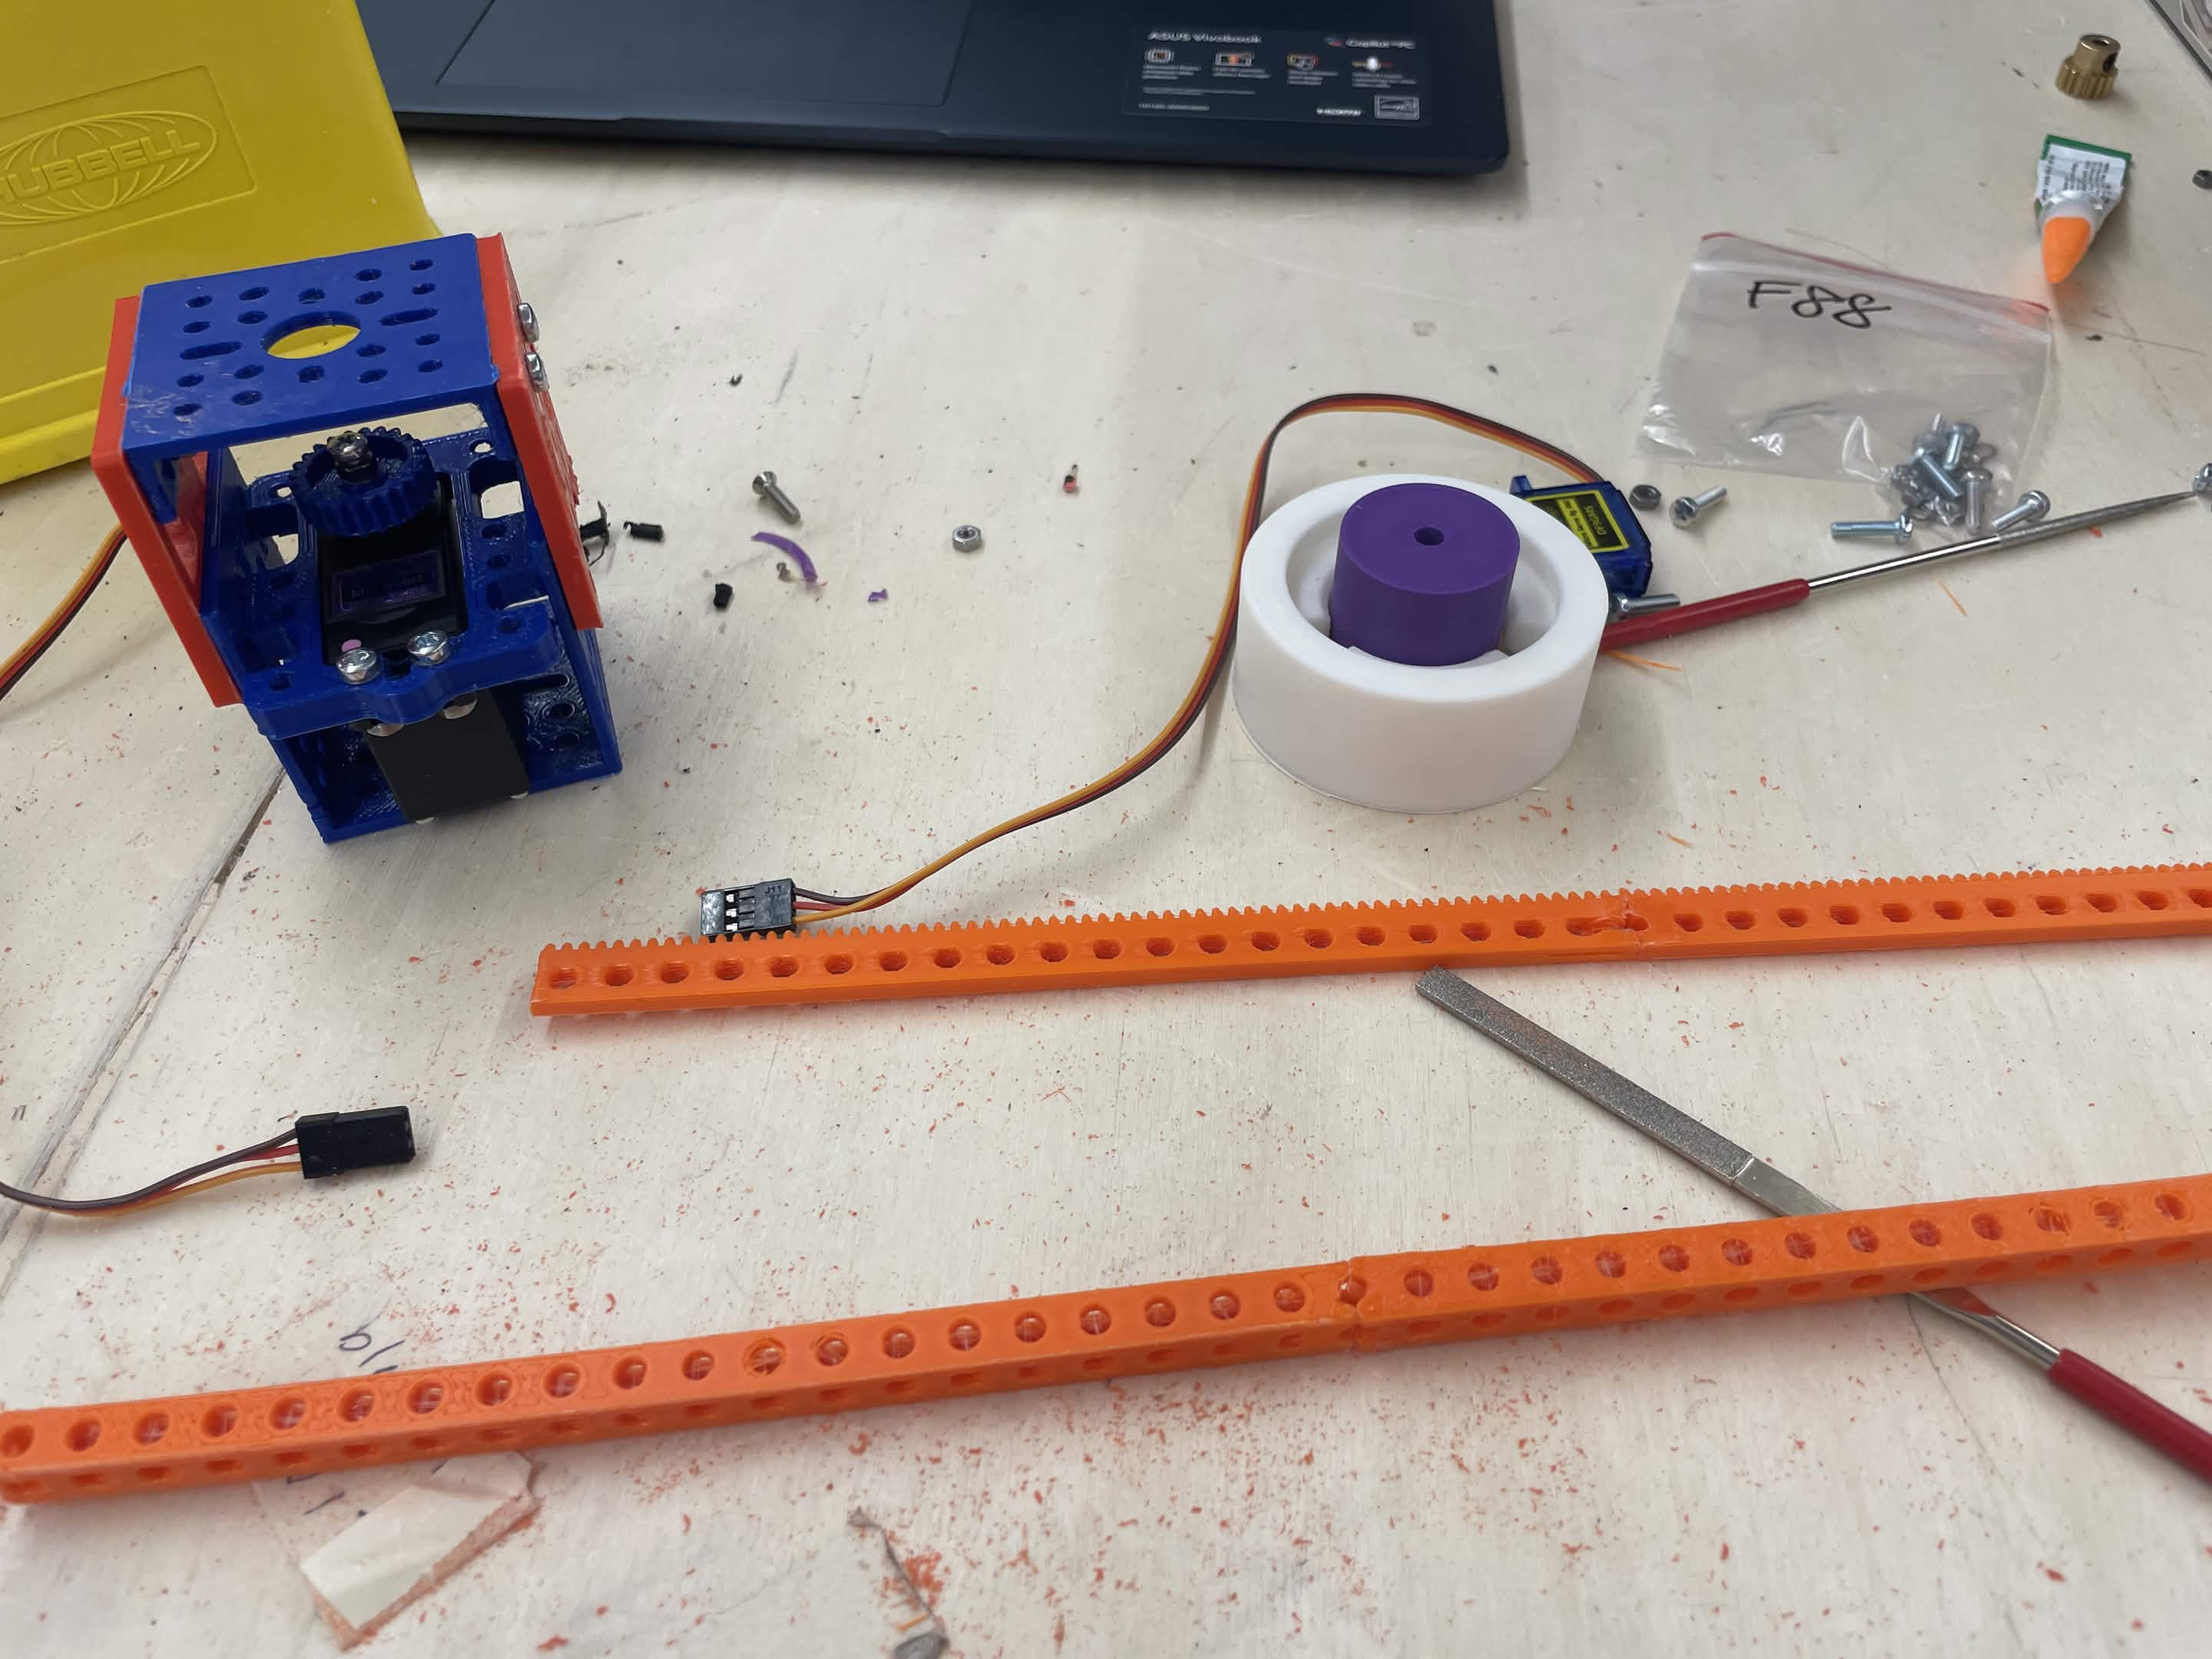
\includegraphics[width=0.7\textwidth]{../mech_img/chassis_assembled.jpg}
\caption{Fully assembled chassis before gear rack insertion.}
\label{fig:assembled}
\end{figure}

\subsection{Key Plastic Fit Adjustment}

The deployment key initially did not fit into the key hole on the box, as shown in Figure \ref{fig:doesnotfit}. Since the key is part of the deployment mechanism and the hole is fixed in the box structure, the key geometry had to be adjusted. The plastic key was soldered to reshape and reduce its profile until it seated cleanly into the hole. Figure \ref{fig:solder_plastic} shows the key after this process.

\begin{figure}[H]
\centering
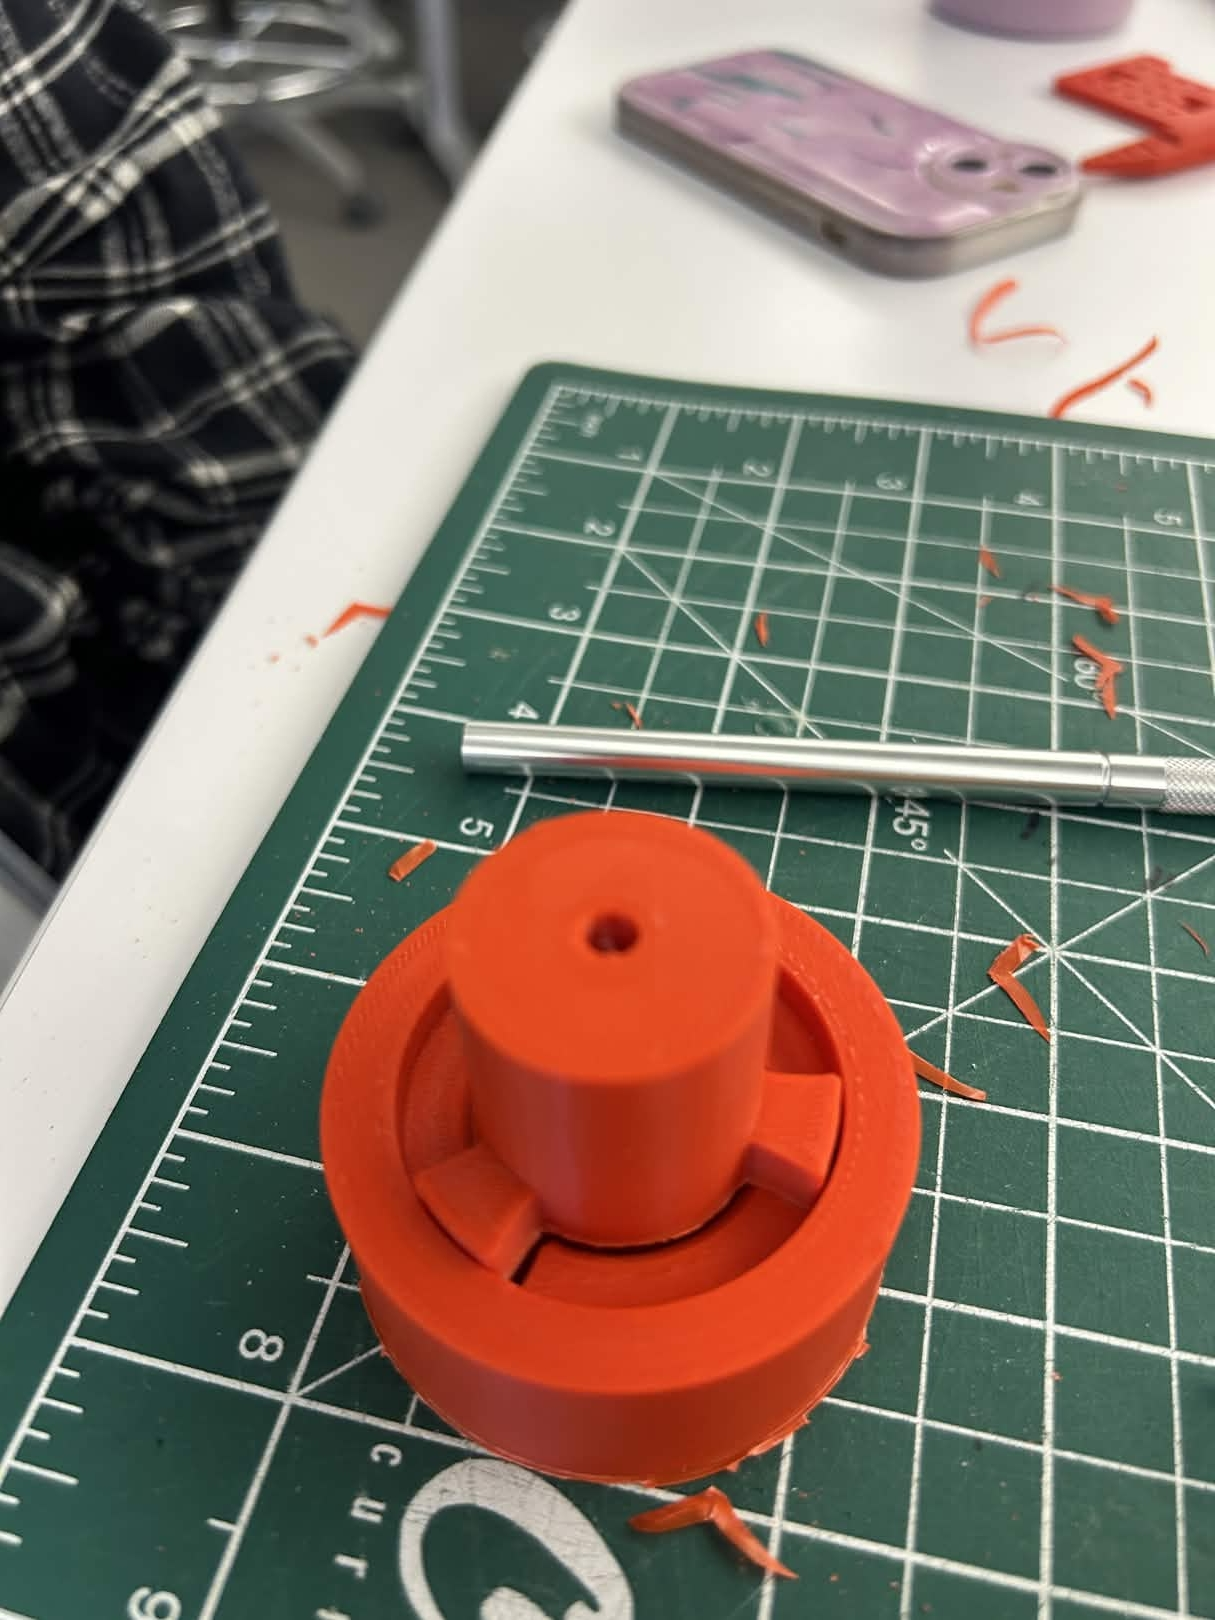
\includegraphics[width=0.65\textwidth]{../mech_img/Does Not Fit.jpg}
\caption{Deployment key initially does not fit into the box key hole.}
\label{fig:doesnotfit}
\end{figure}

\begin{figure}[H]
\centering
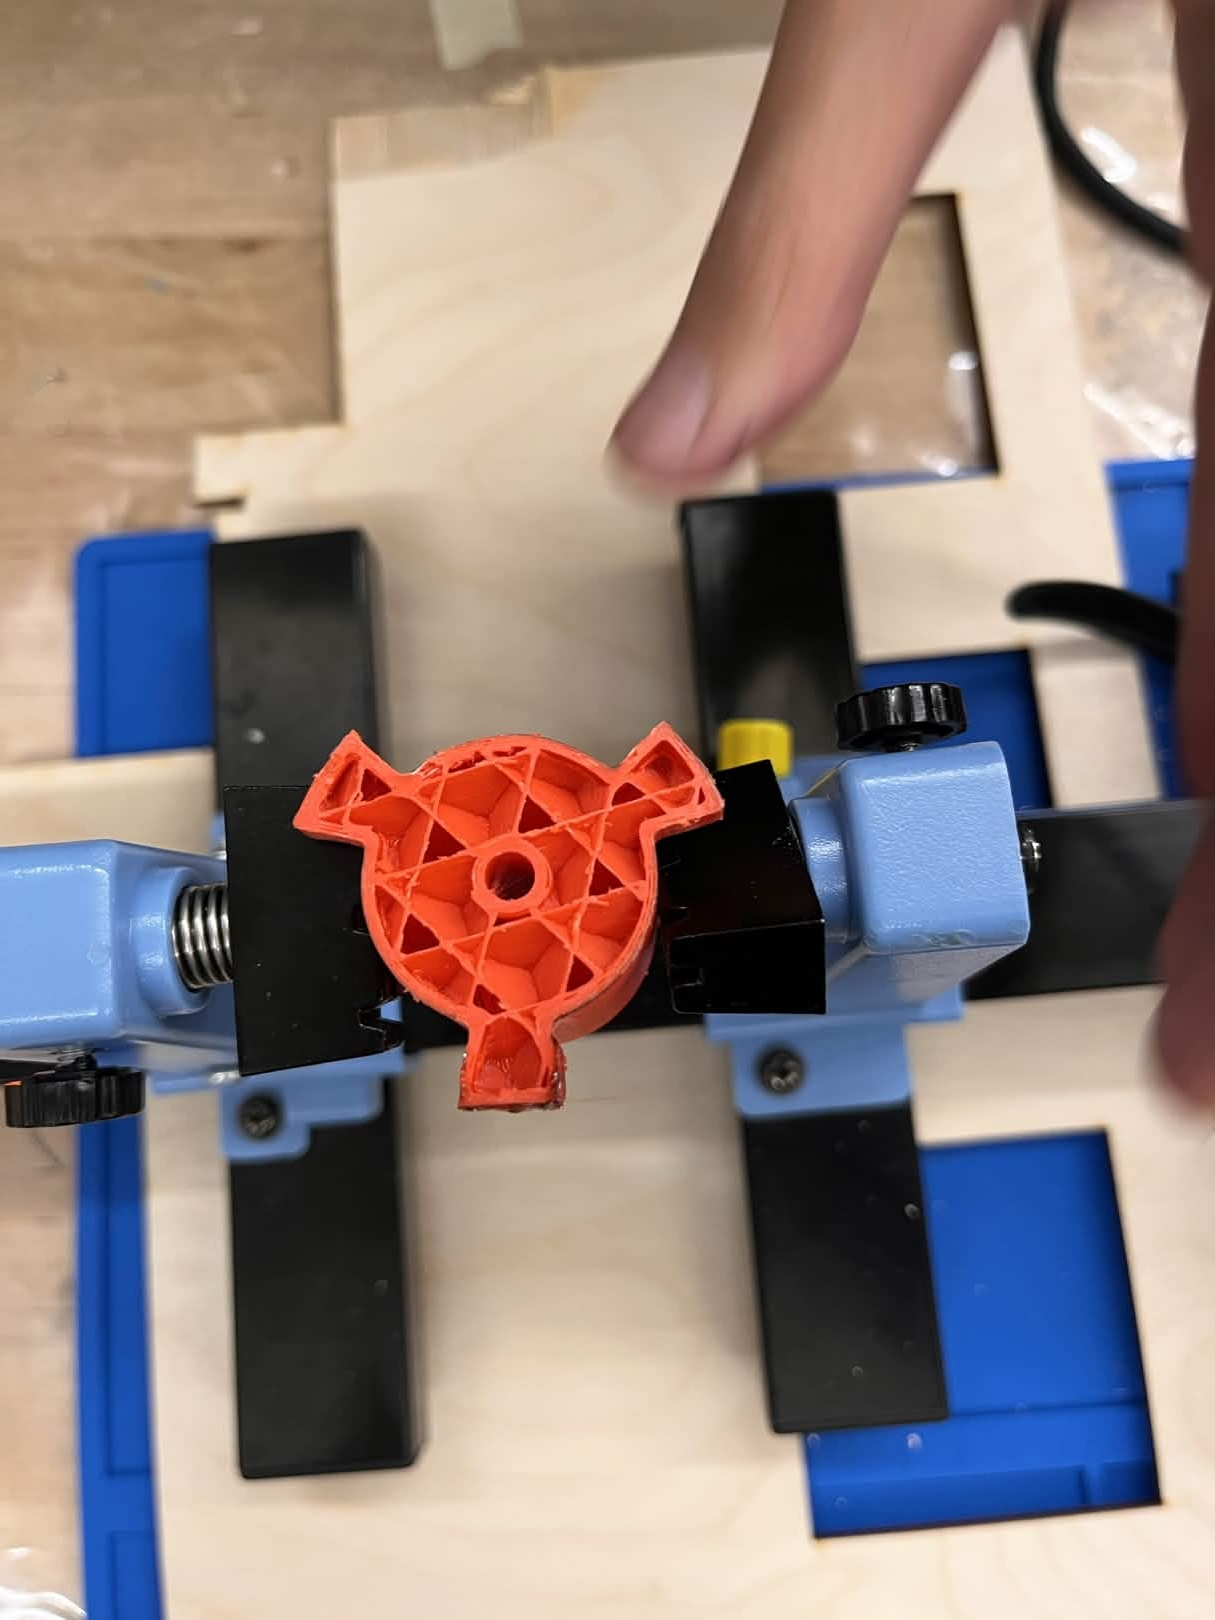
\includegraphics[width=0.65\textwidth]{../mech_img/Solder Plastic 3.jpg}
\caption{Key plastic after soldering to fit into the box key hole.}
\label{fig:solder_plastic}
\end{figure}

\subsection{Final Assembly}

The final integrated prototype is shown in Figure \ref{fig:final}. The gear rack has been inserted through the chassis and properly engaged with the servo-driven gear mechanism. The complete assembly demonstrates the functional deployment system with all mechanical and electrical components integrated.

\begin{figure}[H]
\centering
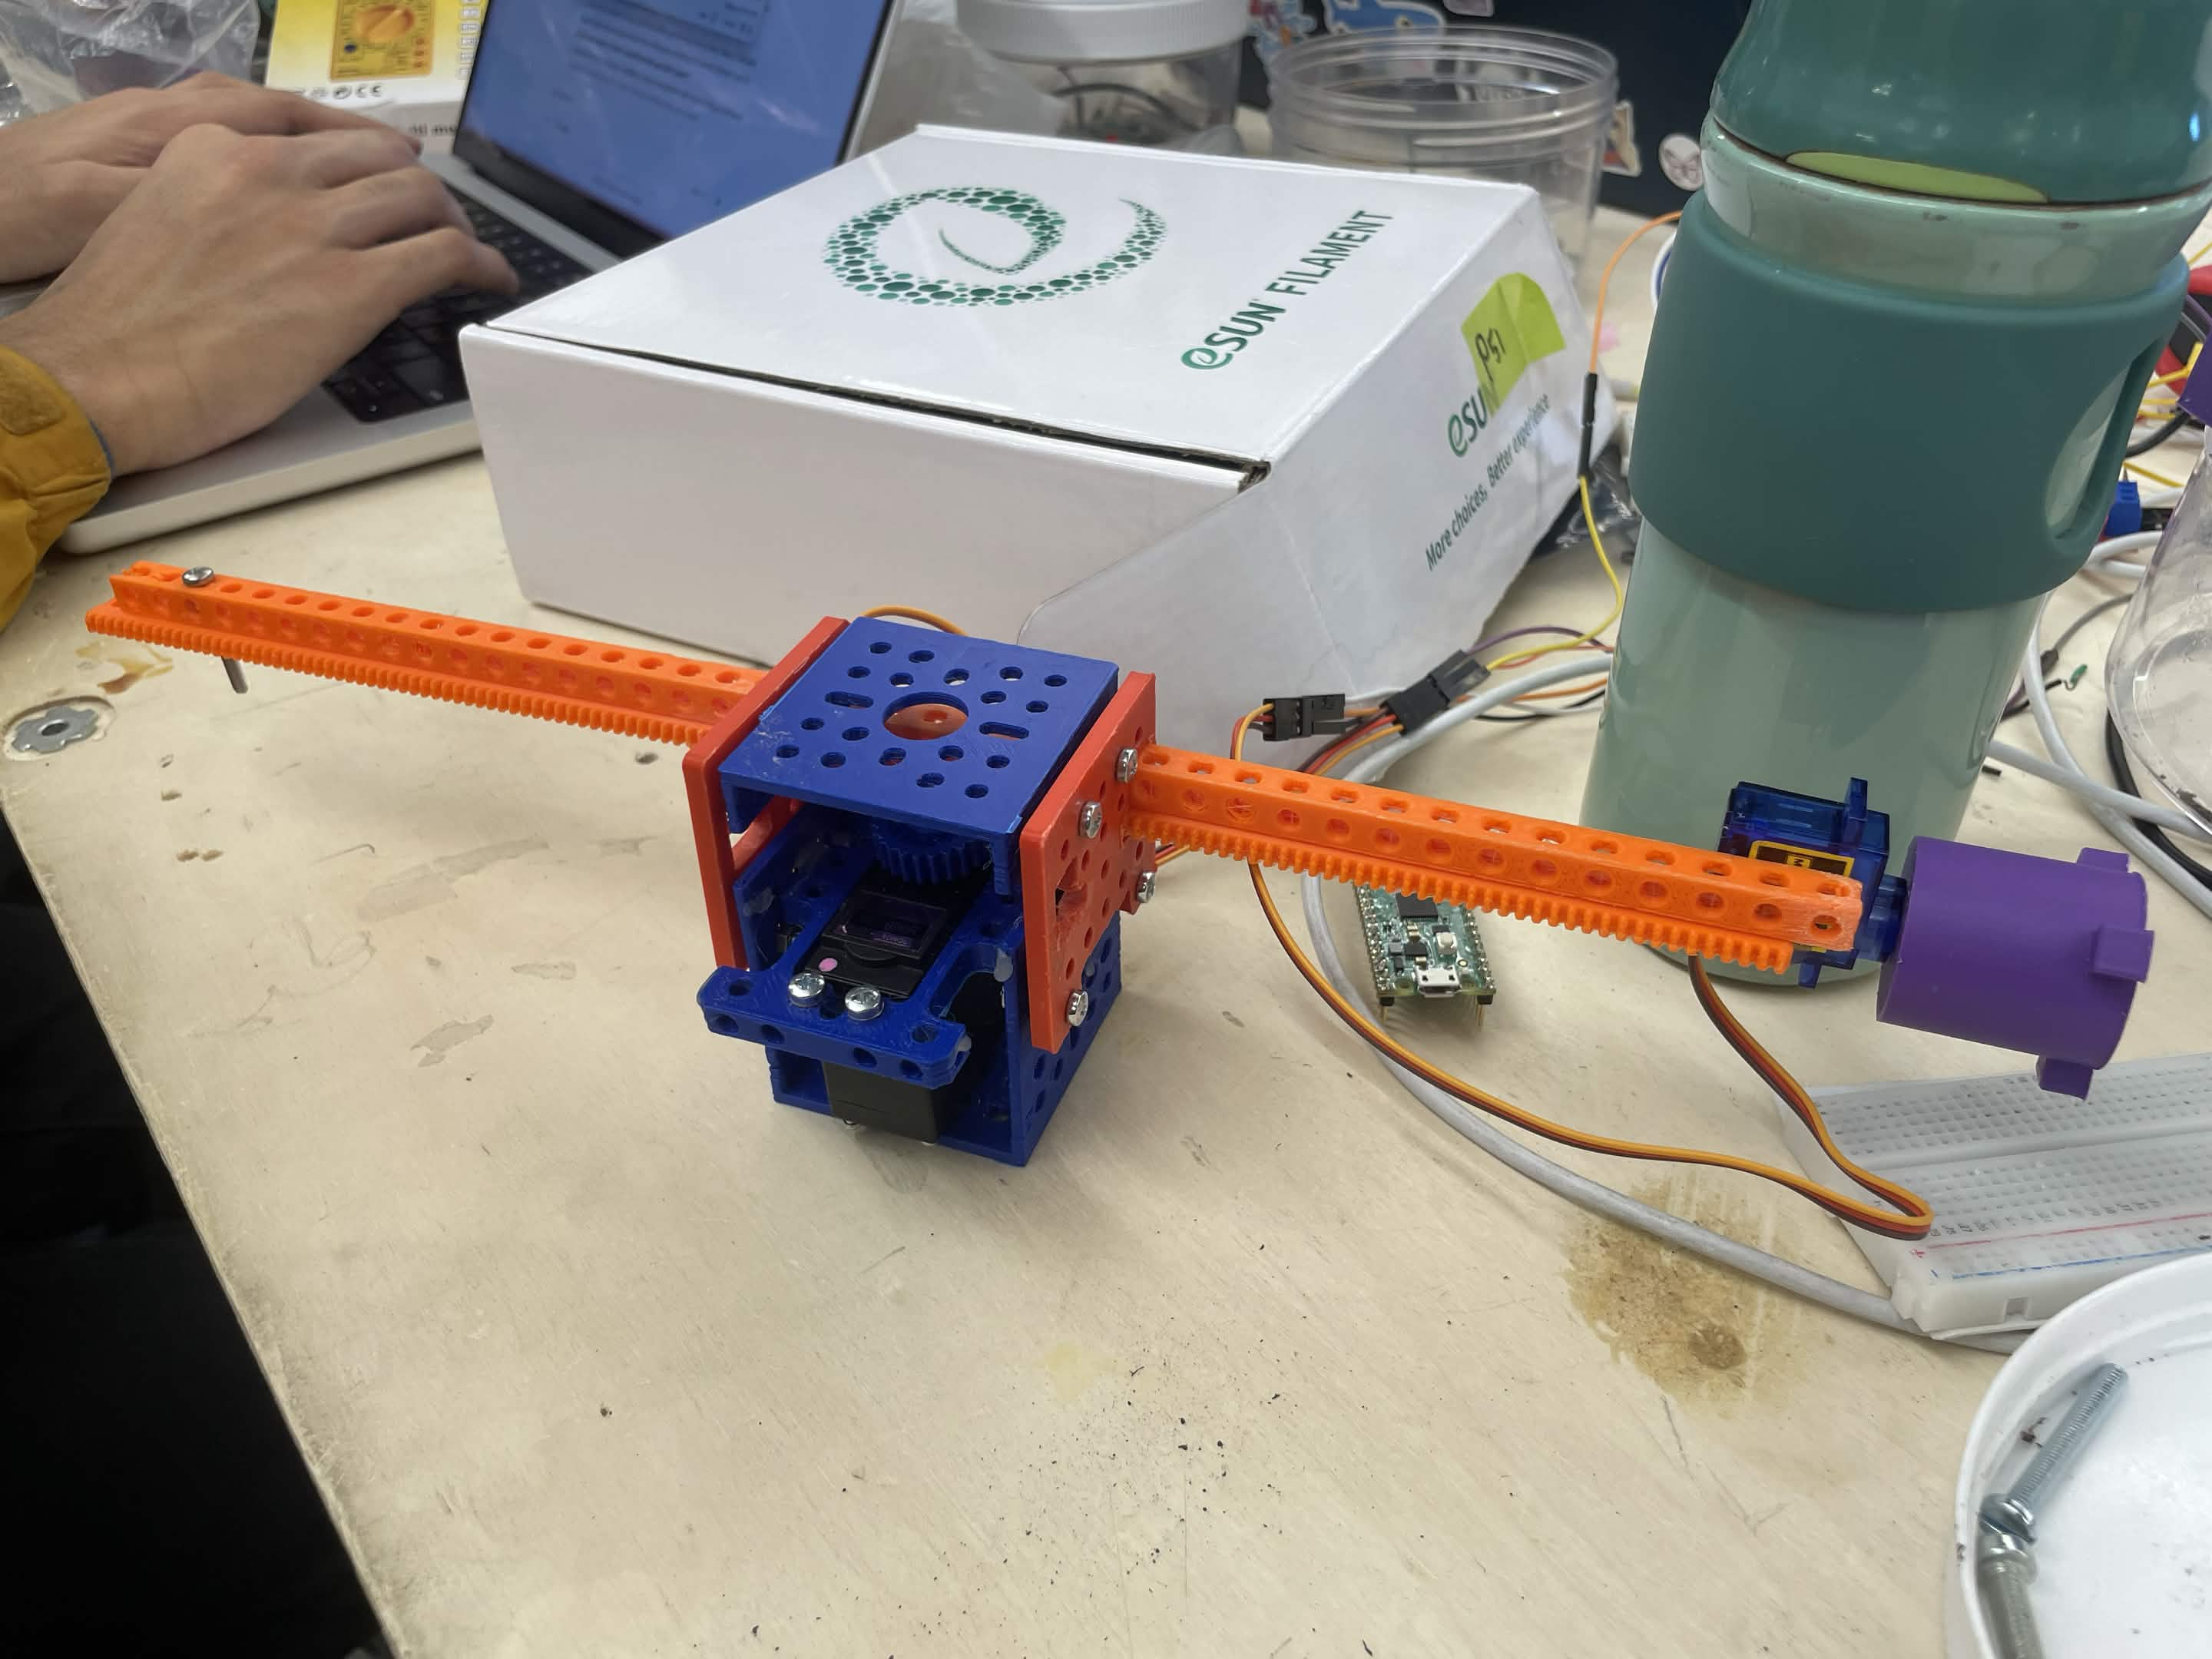
\includegraphics[width=0.7\textwidth]{../mech_img/final_assemble.jpg}
\caption{Final assembled prototype with gear rack integrated into the deployment chassis.}
\label{fig:final}
\end{figure}

\section{Conclusion}

The mechanical assembly of the deployment system was completed through a systematic fabrication process. Initial fit issues with the gear rack were resolved through manual modification, and the deployment key plastic was soldered to achieve a proper fit with the box key hole. All structural components were successfully assembled and secured. The final prototype integrates the chassis, servo motors, and gear rack mechanism into a functional deployment system ready for testing.

\end{document}
